\section{Benchmark}
\label{sec:benchmark}
This section is a comparative description of the results from the sequence classification task described in \autoref{subsec:benchmark-implementation}.
For every benchmark of three epochs precision, recall and F1 are given.
Precision reflects the amount of correct predictions a model has made for that particular class.
Recall shows how often the model correctly predicts a class in relation to all positive predictions.
F1 is a score compromising precision and recall through the \textit{harmonic mean} of precision and recall, measuring the models accuracy.

There is a common trend in all runs displaying a growth in precision, recall and F1.
This means that all models have continously improved predicting the class of a news title.
The highest F1 in the last epoch achieved for any of the smaller models (mso5, msg5, mwo5, mwg5) is mwo5 with a score of 0.69194 (\autoref{tab:mwo5}).
Meanwhile, the lowest F1 is found in \autoref{tab:mwg5} at 0.590542 mwg5.
A similar arrangement is found when comparing final test scores in the set of smaller models: mwo5 > mso5 > msg5 > mwg5 ($0.442827 > 0.405168 > 0.392490 > 0.389116$).

\begin{table}[H]
    \centering
    \caption[Metrics for model mwo5]{Metrics for masked language model trained on the Oscar dataset with Wordmap infused  tokenization. Evaluated on sequence classification task.}
    \label{tab:mwo5}
    \begin{tabular}{lrrlr}
        \toprule
        \textbf{mwo5} & \textbf{Epoch 1} & \textbf{Epoch 2} & \textbf{Epoch 3} & \textbf{Test score} \\
        \midrule
        Precision & 0.292614 & 0.446338 & 0.71387 & 0.449735 \\
        Recall & 0.329531 & 0.552598 & 0.73384 & 0.474525 \\
        F1 & 0.242739 & 0.473851 & 0.69194 & 0.442827 \\
        \bottomrule
    \end{tabular}
\end{table}

Of all small models, mwo5 has the best results for all three metrics precision, recall and F1.
It seemingly learns the fastest out of the four, starting with a recall of 0.329521  and ending on 0.73384 on the last epoch, overtaking its standard counterpart mso5 at the second epoch.

\begin{table}[H]
    \centering
    \caption[Metrics for model mwg5]{Metrics for masked language model trained on the GerParCor dataset with Wordmap infused tokenization. Evaluated on sequence classification task.}
    \label{tab:mwg5}
    \begin{tabular}{lrrrr}
        \toprule
        \textbf{mwg5} & \textbf{Epoch 1} & \textbf{Epoch 2} & \textbf{Epoch 3} & \textbf{Test score} \\
        \midrule
        Precision & 0.237664 & 0.399781 & 0.603534 & 0.441891 \\
        Recall & 0.244613 & 0.463878 & 0.637516 & 0.440304 \\
        F1 & 0.163024 & 0.389905 & 0.590542 & 0.389116 \\
        \bottomrule
    \end{tabular}
\end{table}

Contrary to the pattern of mwo5, the wordmap model trained on GerParCor data predicts less accurately than the standard msg5 model.
The inital epoch shows the lowest scores of all models for precision, recall and logically F1.
None of the predictions keep up with the accuracy of the other small model at any point in training.

\begin{table}[H]
    \centering
    \caption[Metrics for model mso5]{Metrics for masked language model trained on the GerParCor dataset with \ac{bbgc} tokenization. Evaluated on sequence classification task.}
    \label{tab:mso5}
    \begin{tabular}{lrrrr}
        \toprule
        \textbf{mso5} & \textbf{Epoch 1} & \textbf{Epoch 2} & \textbf{Epoch 3} & \textbf{Test scores} \\
        \midrule
        Precision & 0.269615 & 0.422096 & 0.596987 & 0.395879 \\
        Recall & 0.351077 & 0.501901 & 0.657795 & 0.446388 \\
        F1 & 0.266260 & 0.412598 & 0.604824 & 0.405168 \\
        \bottomrule
    \end{tabular}
\end{table}

With an F1 of 0.604824 at the final epoch mso5 is the lowest scoring standard model, despite starting with similar scores in epoch 1 (\autoref{tab:mso5} vs. \autoref{tab:msg5}).
The standard F1 test scores are close to each other, deviating only by one second decimal point indicating comparable benchmark performance.
A comparison with the scores of the other Oscar-trained model mwo5 shows a bigger difference in accuracy, favoring the Wordmap version.
The msg5 iteration is has a slightly steeper adaptation to the task, but fails to carry its performance over to the test scores:

\begin{table}[H]
\centering
\caption[Metrics for model msg5]{Metrics for masked language model trained on the GerParCor dataset with \ac{bbgc} tokenization. Evaluated on sequence classification task.}
\label{tab:msg5}
\begin{tabular}{lrrrr}
    \toprule
    \textbf{msg5} & \textbf{Epoch 1} & \textbf{Epoch 2} & \textbf{Epoch 3} & \textbf{Test scores} \\
    \midrule
    Precision & 0.297466 & 0.517110 & 0.656808 & 0.439873 \\
    Recall & 0.359949 & 0.544994 & 0.676806 & 0.439924 \\
    F1 & 0.267111 & 0.480420 & 0.626593 & 0.392490 \\
    \bottomrule
\end{tabular}
\end{table}

As can be seen, msg5 converges more quickly than its oscar standard counterpart (\autoref{tab:msg5}).
Although it has better precision, recall and F1 throughout all epochs final its test F1 is minimally inferior to mso5.

\begin{table}[H]
    \centering
    \caption[Metrics for model bbgc]{Metrics for masked language model baseline bert-base-german-cased. Evaluated on sequence classification task.}
    \label{tab:bert-base-german-cased}
    \begin{tabular}{lrrrr}
        \toprule
        \textbf{bbgc} & \textbf{Epoch 1} & \textbf{Epoch 2} & \textbf{Epoch 3} & \textbf{Test scores} \\
        \midrule
        Precision & 0.646150 & 0.768675 & 0.860180 & 0.622436 \\
        Recall & 0.709759 & 0.804816 & 0.883397 & 0.637262 \\
        F1 & 0.660588 & 0.778371 & 0.868166 & 0.624789 \\
        \bottomrule
    \end{tabular}
\end{table}

Of all models tested, bert-base-german-cased achieved the highest scores in all categories (\autoref{tab:bert-base-german-cased}).
Its first epoch scores are as high as most of the smaller models final epoch.
It is the only model that manages to achieve test scores above 0.5, but unlike the smaller models also performs below its first epoch scores.

\begin{table}[H]
    \centering
    \caption{Test score summary for all evaluated models.}
    \label{tab:test-summary}
    \begin{tabular}{lrrrrr}
        \toprule
        \textbf{Summary} & \textbf{bbgc} & \textbf{mso5} & \textbf{msg5} & \textbf{wmo5} & \textbf{wmg5} \\
        \midrule
        Precision & \textbf{0.622436} & 0.395879 & 0.439873 & 0.441891 & 0.449735 \\
        Recall & \textbf{0.637262} & 0.446388 & 0.439924 & 0.440304 & 0.474525 \\
        F1 & \textbf{0.624789} & 0.405168 & 0.392490 & 0.389116 & 0.442827 \\
        \bottomrule
    \end{tabular}
\end{table}

\autoref{tab:test-summary} summarizes the final test scores for all evaluated models.
All small model scores are relatively close to each other, but ultimately outperformed by their baseline model for around 0.2 points.
Wmg5 comes closest to the baseline model performance at 0.442827 with a difference of 0.181962.
It beats the smaller model test scores by a small margin of 0.4.


\section{Wordmapping}
\label{sec:wordmapping}

The Wordmap algorithm calculated segment thresholds for each given verb and split the segments into two vocabularies, functional and lexemic.
Sample results for mappings of tokens \textquotesingle viertelt\textquotesingle and \textquotesingle anschauen\textquotesingle are found in \autoref{fig:wordmap2} and \autoref{fig:wordmap3}.:

\begin{figure}[H]
    \centering
    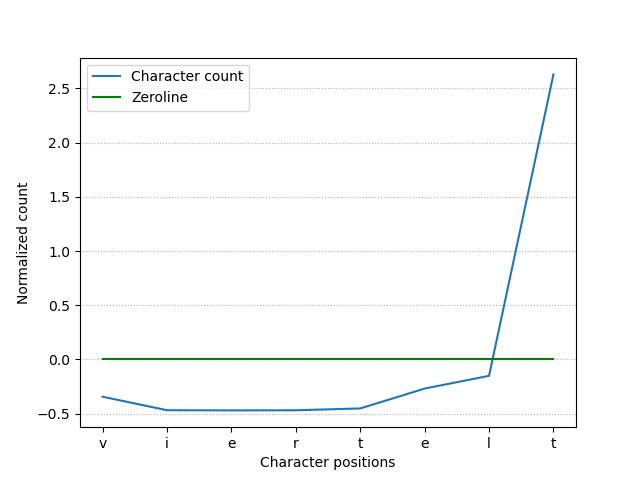
\includegraphics[scale=0.8]{viertelt}
    \caption[Wordmap for \textquotesingle viertelt\textquotesingle]{Wordmap tresholds for token \textquotesingle viertelt\textquotesingle}
    \label{fig:wordmap2}
\end{figure}

\autoref{fig:wordmap2} shows the normalized count of each character relative to the POS corpus.
The Wordmap algorithm interprets \textquotesingle viertelt\textquotesingle as two separate subwords \textquotesingle viertel\textquotesingle and \textquotesingle t\textquotesingle , which correspond to the canonical segmentation of \{viertel\} and \{t\}.
There is a slight fluctuation in lexemic segment ranging between -0.5 and 0 and a strong increase for the functional segment above 2.5 times the standard deviation of counts.

\begin{figure}[H]
    \centering
    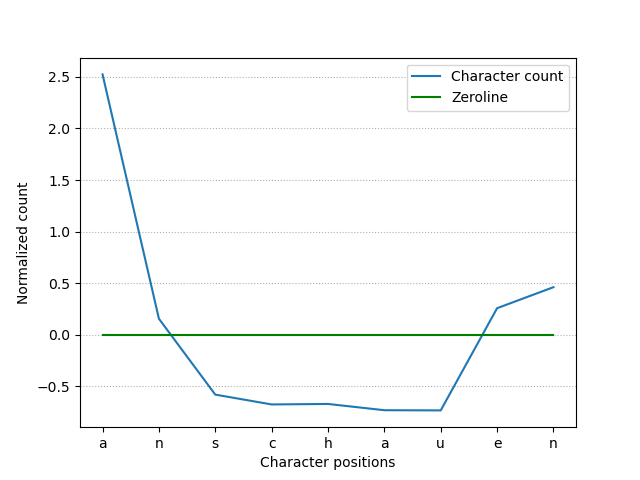
\includegraphics[scale=0.8]{anschauen}
    \caption[Wordmap for \textquotesingle anschauen\textquotesingle]{Wordmap tresholds for token \textquotesingle anschauen\textquotesingle}
    \label{fig:wordmap3}
\end{figure}

The result for the 3-syllabic token \textquotesingle anschauen\textquotesingle is similar, again showing the lexemic part way under the mean count (more than -0.5 standard deviations).
Its prefix \textquotesingle an\textquotesingle and suffix \textquotesingle en\textquotesingle are above zeroline and are thus added to the POS vocabulary.
A difference in affixes can be seen in this example, as the \{an\} combines counts for the morpheme and the single character <a> at the same time.
This part of character bias mentioned in \autoref{subsubsec:generating-a-custom-pre-training-vocabulary} is not captured by the regular expression for character noise reduction.
For every Wordmap, initial and final characters in tokens receive an overall count bias because only those matches are computed in \autoref{alg:wordmap}.
Finally, functional vocabulary holds 138 types of affixes, including subwords, adverbials, prepositions and morphemes found in the german inflection paradigm.
As expected, the lexemic vocabulary contains many more types (over 40k) than the functional one.
Many stems are found multiple time with either subwords or morphemes attached to them.
After combining both vocabularies, a quick search yielded most of the common atomical (non-segmentable) stems like e.g.\ \{schlaf\} and even their changed equivalent \{schlief\}.
The vocabulary was iterated over n^{2} times with different versions of the same verb occuring many times, leading to duplicates.
Ignoring duplicates and duplicate frequency grants a look at the distribution of frequencies in the POS dataset:

\begin{figure}[H]
    \centering
    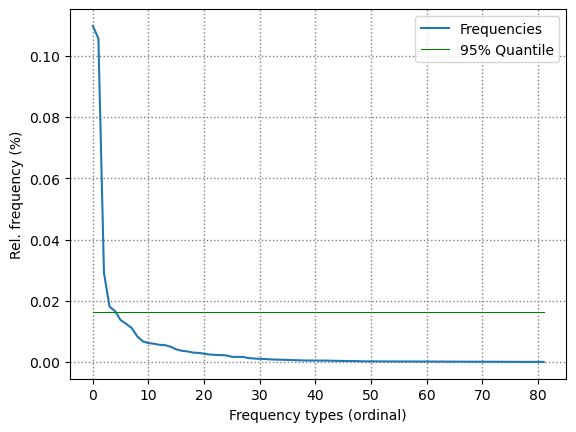
\includegraphics[scale=0.8]{pareto}
    \caption[Pareto distribution in POS vocabulary]{Frequency values mapped to unique frequencies}
    \label{fig:pareto}
\end{figure}

Plotting the relative frequency value to the set of unique frequencies in the POS vocabulary shows a pareto-like disribution (\autoref{fig:pareto}), hinting at Zipf\textquotesingle s law applied to the behavior of frequency in natural language.
The 95\% quantile visualizes the amount of non-frequent subwords contained in the vocabulary - this becomes extremely distorted when plotting tokens to their frequency.

